\title{The Incandescent Lamp and the Inverse Square Law}
\author{An Introduction to Physics through Experiments}
\date{}

\maketitle

\section*{Objectives}

\begin{enumerate}
\item To understand the current-voltage characteristics of an incandescent lamp's filament.
\item To understand the dependence of the lamp's power on the resistance of its filament.
\item To observe and understand the variation of intensity with distance for a point source.
\end{enumerate}




\section*{Apparatus}

\begin{enumerate}
\item A DC variable power supply (\textit{Optochem})
\item Two digital multimeters with probes (\textit{MECO 603} and \textit{Victor VC97})
\item A 12 V, 21W incandescent lamp
\item A stand to hold the lamp
\item A Resistor Ladder
\item Connecting cords
\item A convex lens
\item A photodiode

\end{enumerate}


\section*{Introduction}



\section*{Description}

In \textbf{Part A}, you will design an experiment to study the VI characteristics of an incandescent lamp. 

In \textbf{Part B}, you will design an experiment to observe the variation of the lamp's power with the resistance of its filament. 

In \textbf{Part C}, you will design an experiment to create a point source and then observe the variation of its intensity as a function of the distance from the source. 


\section*{Theory}

\subsection*{Part A}

If an electric current is passed through a wire of significant resistance, the wire will be heated. If the wire is heated to a sufficiently high temperature, it will give off light.  This is the basis of a resistive incandescent lamp. The high melting point of tungsten (3680 K) and its low vaporization pressure makes it a suitable material to be used as the filament of almost all incandescent lamps. The brightness and the overall colour of emitted light depends on the temperature of the filament for a given lamp, which is a non-linear resistive element.

It is observed that (for a specific range of current) almost all incandescent lamps satisfy the relation

\begin{equation*}
V = K I^a
\end{equation*}

where $V$ is the voltage across the lamp, $I$ the current passing through the lamp, and $K$ and $a$ are constants.

\subsection*{Part B}


One finds for the resistive lamp, the empirical relation

\begin{equation*}
P = C R^n
\end{equation*}

where $P$ is the power supplied to the lamp, $R$ is the resistance of the filament of the lamp, and $n$ and $C$ are constants whose values depend on the material used for the filament of the lamp. The above relation yields better results when the temperature of the filament of the lamp is approximately above 1800 K for the given lamp. For such temperatures the resistance R of the lamp is found to be directly proportional to the absolute temperature T of the filament of the lamp.



\subsection*{Part C}


\begin{minipage}{0.5\linewidth}
%\vspace{-1.5cm}
A \textbf{point source} is a single identifiable localised source of, say, light. Such a source has negligible extent, distinguishing it from other source geometries, and are called point sources because in mathematical modeling, they can usually be approximated as a mathematical point to simplify analysis. The actual source need not be physically small, if its size is negligible relative to other length scales in the problem. For example, in astronomy, stars are routinely treated as point sources, even though they are in actuality much larger than the Earth.

For light or sound waves, a point source radiates the same intensity of radiation in all directions. That is, it has no preferred direction of radiation and radiates uniformly in all directions over a sphere centred on the source.
\end{minipage}
\begin{minipage}{0.5\linewidth}
\centering
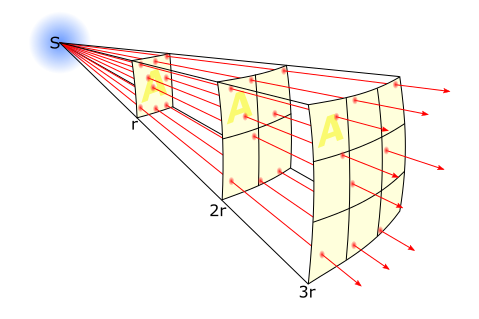
\includegraphics[scale=0.7]{isl.png}
\end{minipage}



\section*{Experimental Setup}

\subsection*{Digital Multimeter (\textit{MECO 603})}

A multimeter is an instrument used to measure multiple parameters like voltage, current, and resistance. In this experiment you are given two digital multimeters (Models \textit{MECO - 603} and \textit{Victor VC97})\footnote{The Victor multimeter has a greater current sensitivity.}. You will have to use input sockets marked COM, V/$\Omega$ and mA (or A or 20A) for the required measurements. Note that there are two input sockets marked mA and 20A (10A for the Victor multimeter) for the current measurement. The socket marked mA may be used for measuring current below 250 mA and socket marked 20A (or 10A) may be used for measuring current up to 20 A (or 10A). You will have to select the appropriate function and the range using the rotary switch provided on the multimeter. The value of voltage or current is displayed on the LCD screen. The multimeter is turned off by turning the dial to the appropriate setting.

\subsection*{Variable DC Power Supply (\textit{Optochem})}

The power switch can be used to switch it ON or OFF. The required output can be taken from the two output terminals. The voltage and the current capacity can be changed using the three knobs: voltage coarse, voltage fine, and current. The given power supply also displays the values of the output voltage and current. Do not use these value since measuring these values using given calibrated multimeter will be more reliable. 

The DC Variable Power Supply can either act as a source of Constant Current (CC) or Constant Voltage (CV). In general, most types of circuits require a constant voltage to operate. The power supply has a physical limit on how much current it can supply, if the load (your circuit) attempts to draw more, the power supply decreases the output voltage to keep the current consumed at its maximum permissible amount. For this experiment, you should turn the current dial up to the maximum. This allows the supply to work as a constant voltage supply unless the current drawn by your circuit goes beyond 2A.

\subsection*{Photodiode}

A photodiode is a semiconductor device that converts light into an electrical current. The current is generated when photons of sufficient energy are absorbed in the photodiode, creating an electron-hole pair through the photoelectric effect.

\subsection*{Warnings}

\begin{enumerate}
\item Do not apply a voltage more than 12 V to the lamp.
\item Clamp the lamp carefully on the retort stand so that it should not be damaged or the wires should not get shorted.
\item You will have to use the given fixed value resistor to control the current in the circuit.
\item Use the digital multimeter for the measurement of D.C. voltage and current.  Choose the most appropriate range for the measurement.
\item The incandescent lamp should not be kept connected to the power supply for long duration. 

\item Passing more current through the multimeter's (250 mA or 20A) sockets than they can handle will cause the fuses in the multimeter to burn out, leading to an open circuit. Use an appropriate resistance to limit the current in the circuit.

\item When drawing circuit diagrams use the standard symbols.

\item The digital multimeter, the DC power supply or the signal generator should be turned off if not in use.

\end{enumerate}


\section*{Procedural Instructions}

\subsection*{Part A}

You have to design and perform an experiment to determine the value of constant a for the given incandescent lamp, given that it follows the equation 

\begin{equation*}
V = K I^a
\end{equation*}

You will have to plot an appropriate graph and from the graph determine the value of $a$. Draw the necessary circuit diagram in your answer sheet.

\paragraph{Question:} How does the resistance of the lamp vary with the current?  Explain the cause of variation of the resistance of the lamp with the current?

\subsection*{Part B}

You have to design an appropriate procedure to determine the value of $n$. You may use the data gathered earlier, or you may perform new measurements. Plot the appropriate graph to determine the value of $n$.

\subsection*{Part C}

In this part, you have to study the fall of intensity of light emitted by the given incandescent lamp.  For this you have to use the given photodiode with a digital multimeter to measure the intensity of light. We assume that the relation between the intensity of light incident on the sensing area of the photodiode and its output current is linear. 

Use the converging lens that we have provided you with in order to create a point source. You may use the screen with a hole in it to allow the passage of a small amount of light of this `point source' that may then be detected by the photodiode. This screen will now act as your source.

Connect the output of the power supply to the given lamp and adjust the voltage applied to the lamp to be around 12 V. Keep the photodiode initially as close as possible to the screen acting as your source.  Study the variation of current IPD in the photodiode with the distance $d$ between the source and the photodiode. (You have to take readings for the value of $d$ varying from around 7.0 cm to around 50.0 cm.) You may have to correct your readings to account for the ambient light falling on the photodiode. 

Plot an appropriate linear graph to show the variation of the intensity of light with distance $d$.

\paragraph{Question:} What type of graph would be the most efficient to determine the variation of the intensity of light with distance?

\paragraph{Question:} After plotting this graph, you may find that points below 20.0 cm do not behave as you would expect them to. Can you explain why this is the case?


\section*{References}

\begin{enumerate}

\item \href{https://www.fh-muenster.de/ciw/downloads/personal/juestel/juestel/4-InkohaerenteLichtquellen-Glueh-_und_Halogenlampen_english_-1.pdf}{Incandescent and Halogen Lamps}

\item \href{https://www.elprocus.com/photodiode-working-principle-applications/}{Photodiode Working Principle, Characteristics and Applications}

\end{enumerate}